\documentclass[12pt]{article}
\usepackage[english]{babel}
\usepackage{natbib}
\usepackage{url}
\usepackage[utf8x]{inputenc}
\usepackage{amsmath}
\usepackage{graphicx}
\graphicspath{{images/}}
\usepackage{parskip}
\usepackage{fancyhdr}
\usepackage{vmargin}
\usepackage{xcolor}
\usepackage{siunitx}
\usepackage{physics}
\setmarginsrb{3 cm}{2 cm}{3 cm}{2 cm}{1 cm}{1.5 cm}{1 cm}{1.5 cm}

\title{Lab 04}													% Title
\author{G 03}														% Author
\date{8 Apr 2019}														% Date

\makeatletter
\let\thetitle\@title
\let\theauthor\@author
\let\thedate\@date
\makeatother

\pagestyle{fancy}
\fancyhf{}
\rhead{\theauthor}
\lhead{\thetitle}
\cfoot{\thepage}
\newcommand{\mis}[3]{(#1 \pm #2) \ #3}
\newcommand{\misp}[3]{(#1 \#3 \pm #2}
\begin{document}

%%%%%%%%%%%%%%%%%%%%%%%%%%%%%%%%%%%%%%%%%%%%%%%%%%%%%%%%%%%%%%%%%%%%%%%%%%%%%%%%%%%%%%%%%

\begin{titlepage}
	\centering
    \vspace*{0.5 cm}
    
\includegraphics[scale = 0.75]{polito.jpg}\\[1.0 cm]				% University Logo
    \textsc{\LARGE Politecnico di Torino}\\[2.0 cm]						% University Name
	\textsc{\Large Digital systems electronics\\ A.A. 2018/2019}\\[0.5 cm]		% Course Code
	\textsc{\Large Prof. G. Masera}\\[0.5 cm]		% Nome del Professore
	\rule{\linewidth}{0.2 mm} \\[0.4 cm]
	{ \huge \bfseries \thetitle \\ \small \thedate}\\
	\rule{\linewidth}{0.2 mm} \\[1.5 cm]
	
	\begin{minipage}{0.4\textwidth}
		\begin{flushleft} \large
			Berchialla Luca\\												%Cognomi e nomi
			Laurasi Gjergji
			\\
			
			Mattei Andrea\\
            Lombardo Domenico Maria\\
            
			\end{flushleft}
			\end{minipage}~
			\begin{minipage}{0.4\textwidth}
            
			\begin{flushright} \large
			236032\\													%Matricole
			238259\\
            233755\\
            233959\\
            
		\end{flushright}
        
	\end{minipage}\\[2 cm]
	
\end{titlepage}

%%%%%%%%%%%%%%%%%%%%%%%%%%%%%%%%%%%%%%%%%%%%%%%%%%%%%%%%%%%%%%%%%%%%%%%%%%%%%%%%%%%%%%%%%
\newpage

\section{Gated SR latch}

The circuit shown in $figure\;1$ implements a gated SR latch.
Once coded into VHDL the Quartus Prime compiler uses separate memory components as shown in $figure\;2$ to depict the electric circuit.

\begin{figure}[h]
	\centering
    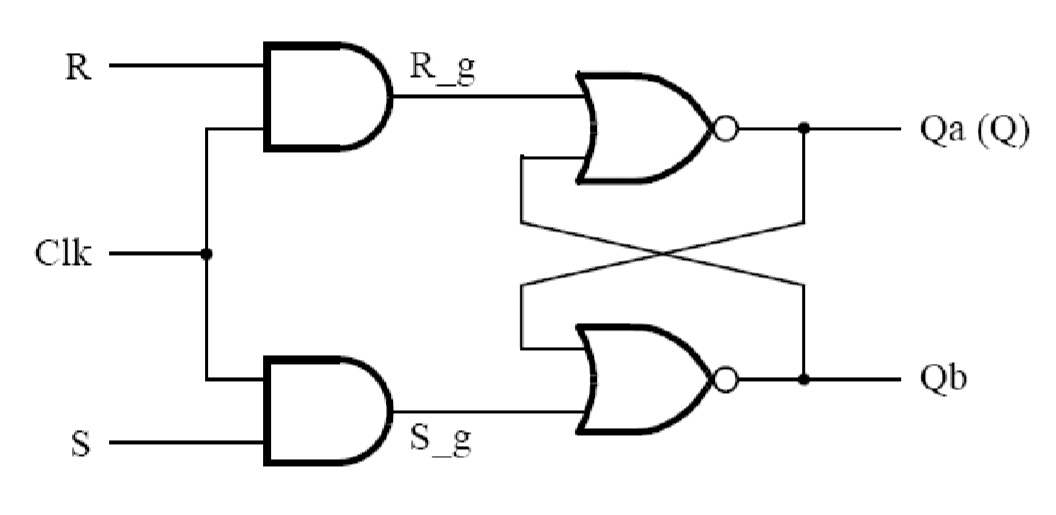
\includegraphics[scale = 0.75]{immagini/SRff.PNG}
    \caption{A gated SR latch circuit}		
\end{figure}

\begin{figure}[h]
	\centering
	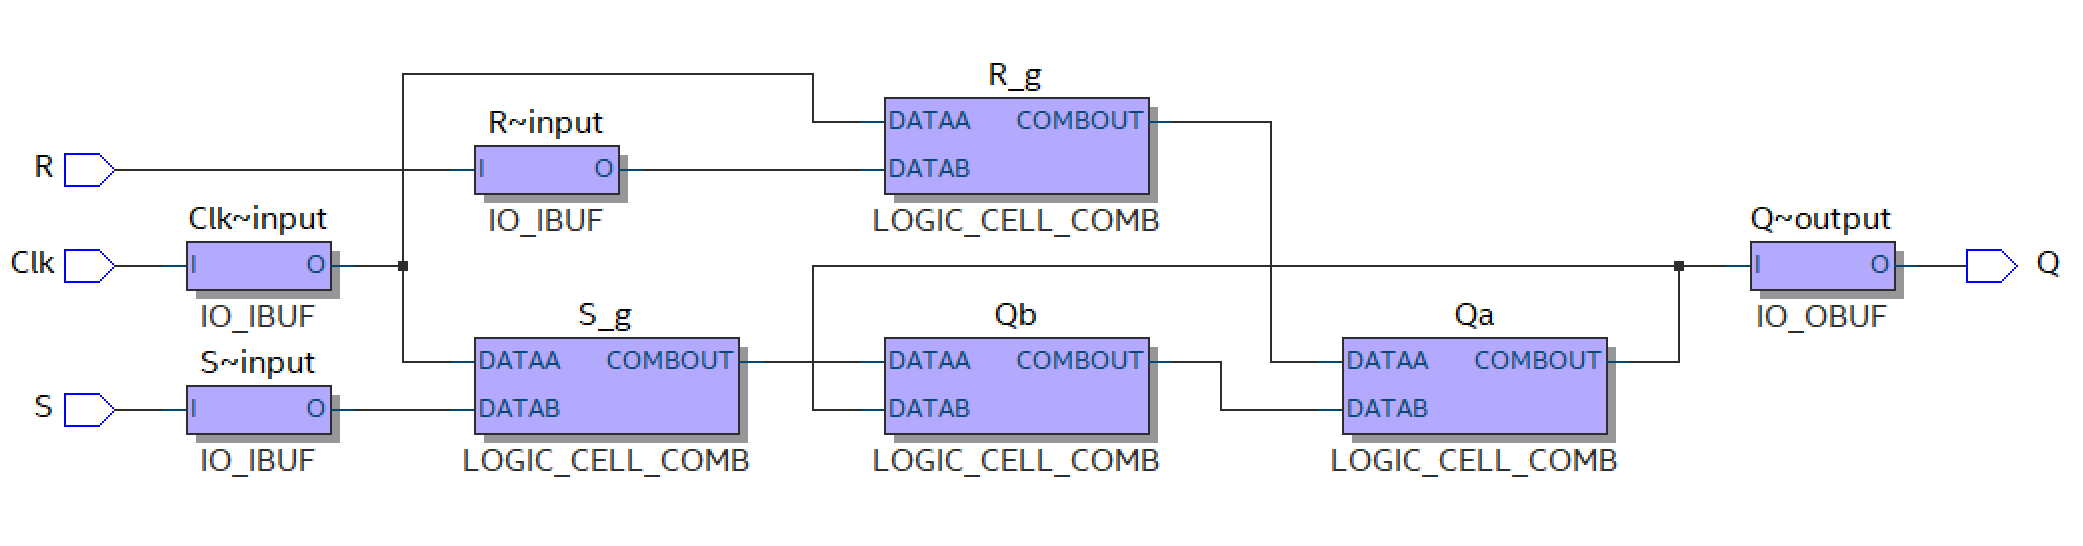
\includegraphics[scale = 0.6]{immagini/postmap.PNG}
	\caption{Quartus circuit implementation}
\end{figure}
\vspace{5mm}
\newpage
Finally, a testbench has been written to test the behavior of the circuit, according to the table shown below:
\vspace{5mm}
\begin{figure}[h]
	\centering
	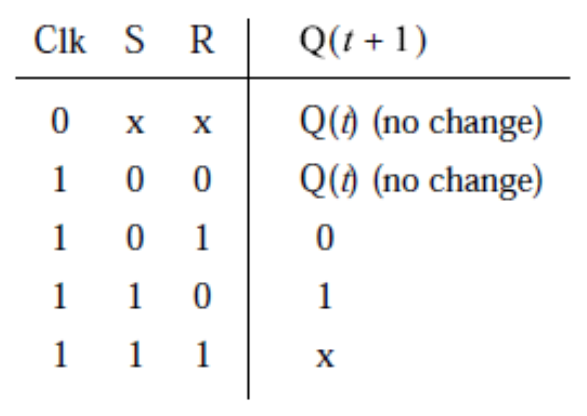
\includegraphics[scale = 0.6]{immagini/table_sr.PNG}		
\end{figure}


\begin{figure}[h]
	\centering
	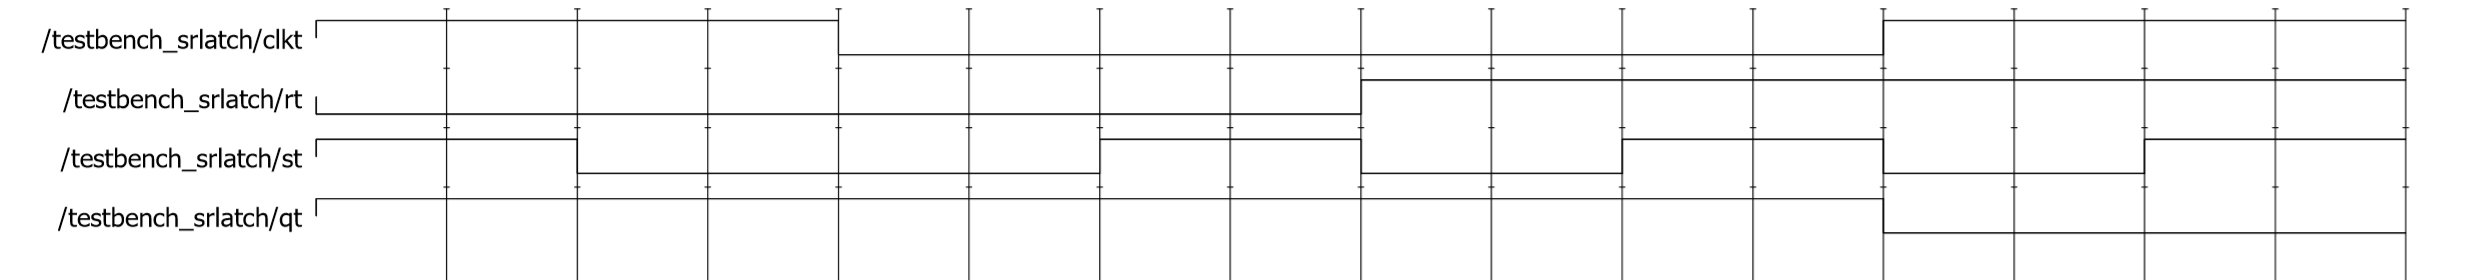
\includegraphics[scale = 0.45]{immagini/testbench1.PNG}
	\caption{Modelsim Testbench waves}
\end{figure}
The testbench results are shown by means of the simulated waves shown in $figure\;3$. 
Initially $CLK=1$, the lath is enabled. For $S=1$, $R=0$ the set condition is triggered and $Q=1$. Viceversa $Q=0$ when $S=0$, $R=1$, in reset condition. Once $CLK=0$ the latch is disabled entering in the memory condition as $S=0$, $R=0$. In the other hand for $S=1$, $R=1$ the latch behavior becomes unpredictable.
\vspace{10mm}
\newpage
\section{16-bit synchronous counter}

The circuit in $figure\;4$ implements a 4-bit counter using T flip flops. A 16-bit version has been implemented using the same structure as shown in figure 5. Using the Quartus tools the maximum working frequency has been identified to be equal to $F=374.53MHz$ as reported in $figure\;5$ using a total of $31$ LEs.

 In the implementation of the 16-bits counter respect to the 4-bit counter no differences as observed in terms of architecture.




\vspace{10mm}
\begin{figure}[h]
	\centering
	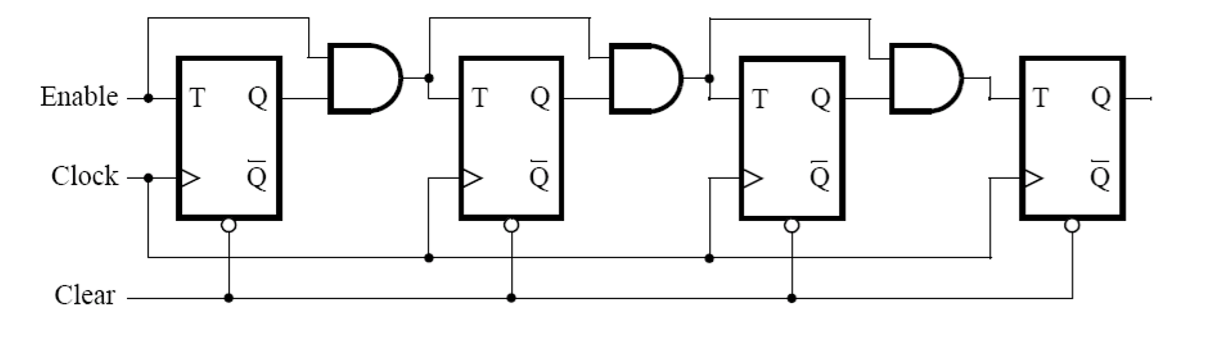
\includegraphics[scale = 0.8]{immagini/count.PNG}
	\caption{4-bit counter}
\end{figure}

\begin{figure}[!h]
	\centering
	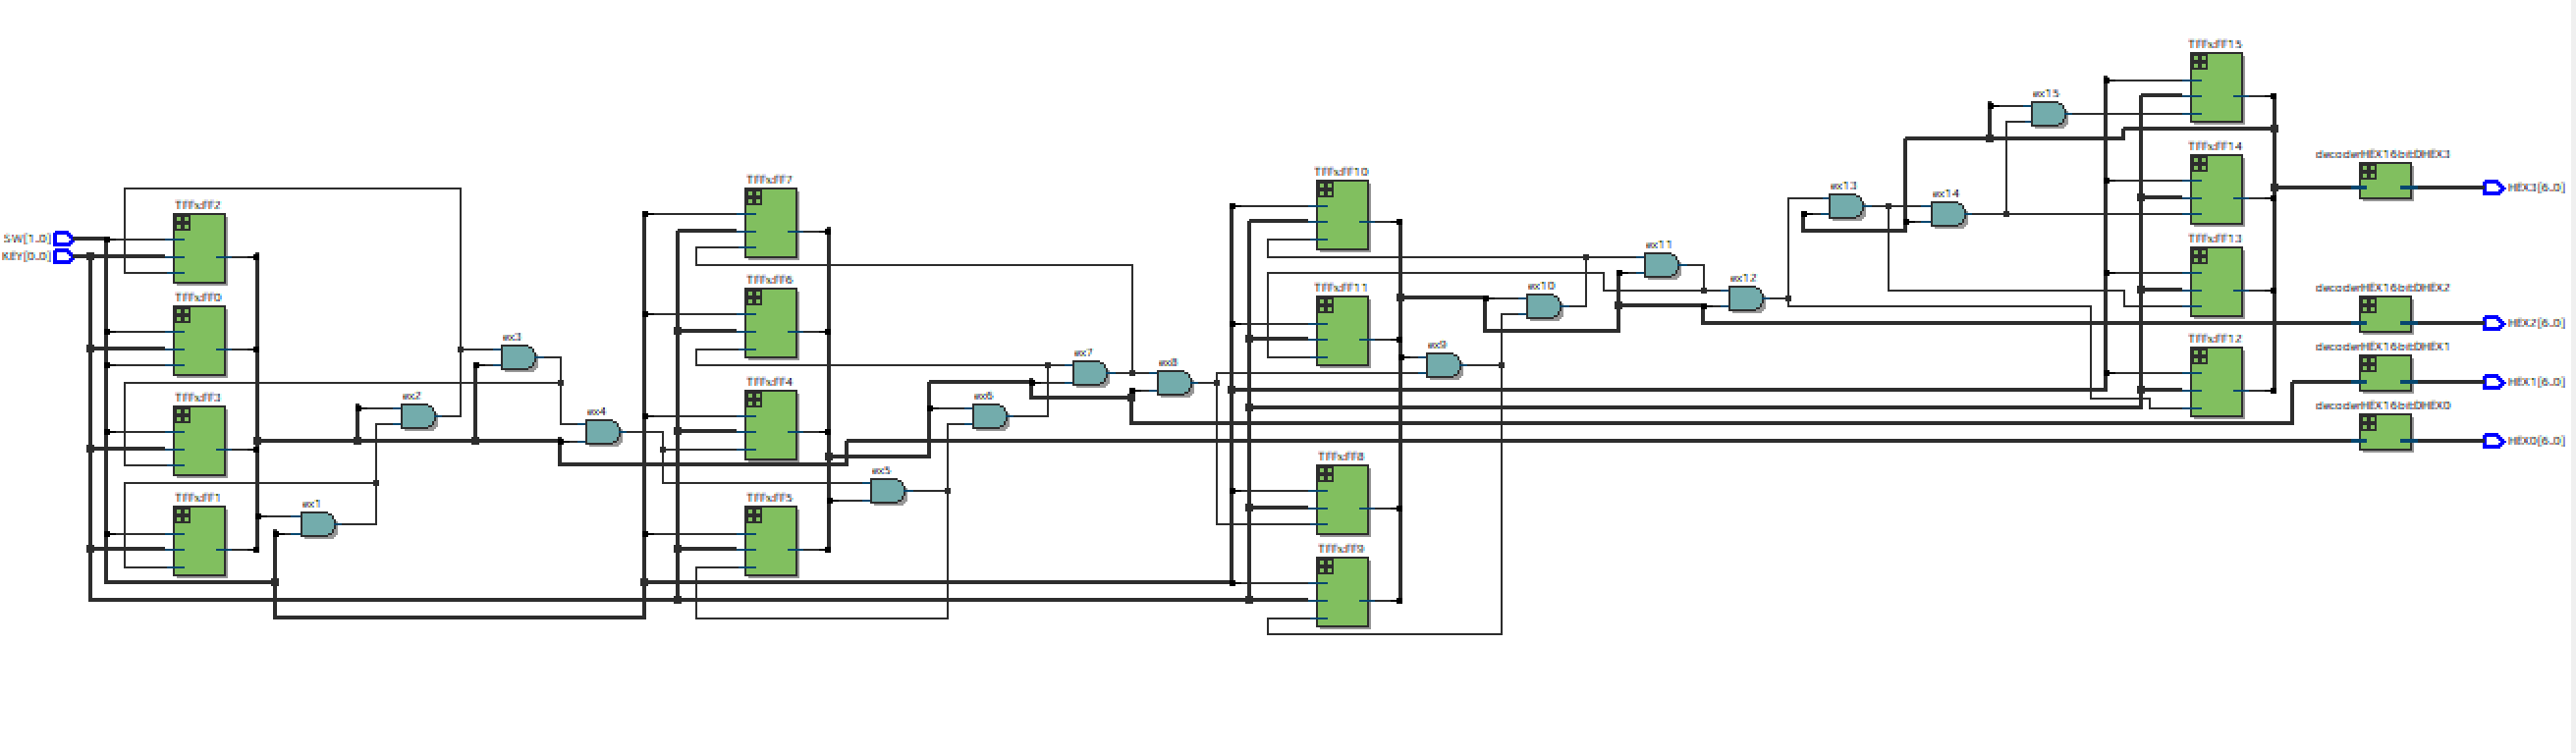
\includegraphics[scale = 0.4]{immagini/immagine42.PNG}
	\caption{4-bit counter}
\end{figure}
\vspace{10mm}
	\begin{figure}[h]
		\centering
		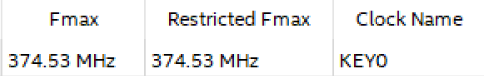
\includegraphics[scale = 0.9]{immagini/fmax.PNG}
		\caption{Maximum working frequency}
	\end{figure}
\newpage
Finally a testbench has been designed to check the functionality of the circuit, the results are shown in $figure\;6$ where the counting process is shown using the HEX display. Notice that the circuit is firstly initialized resetting the current state of every FF. Then the counting process has been started enabling the circuit and applying a clock to every FF.
		\begin{figure}[h]
			\centering
			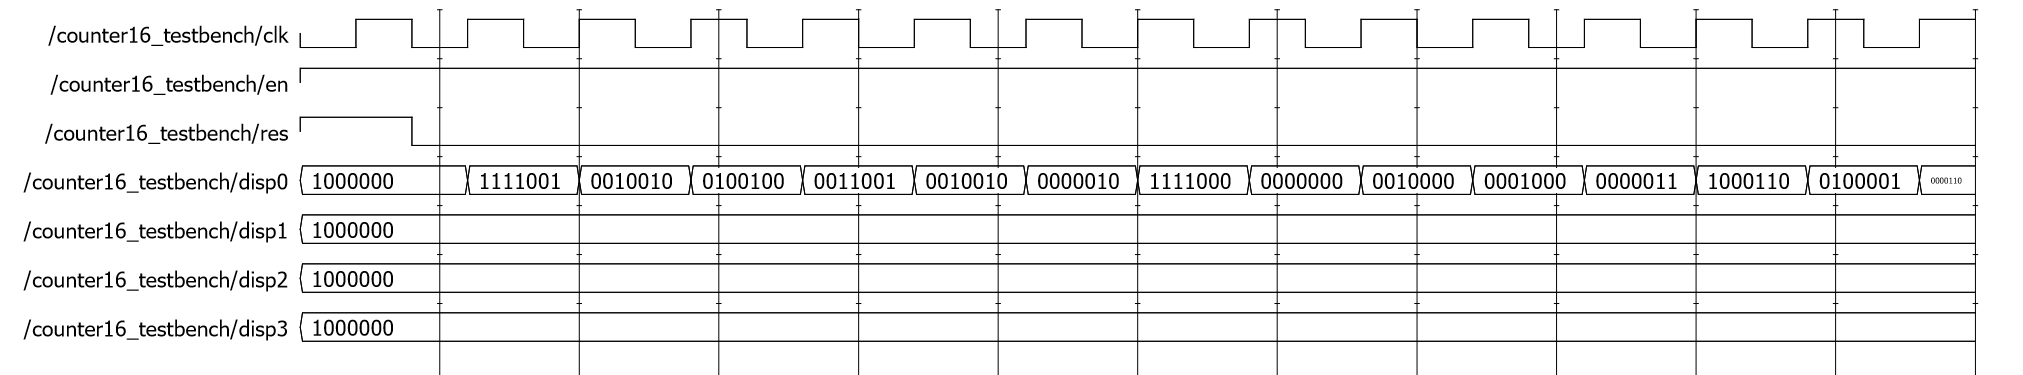
\includegraphics[scale = 0.6]{immagini/testbench2.PNG}
			\caption{Modelsim Testbench waves}
\end{figure}
\section{16-bit synchronous counter version 2}
9LEs
\begin{figure}[h]
	\centering
	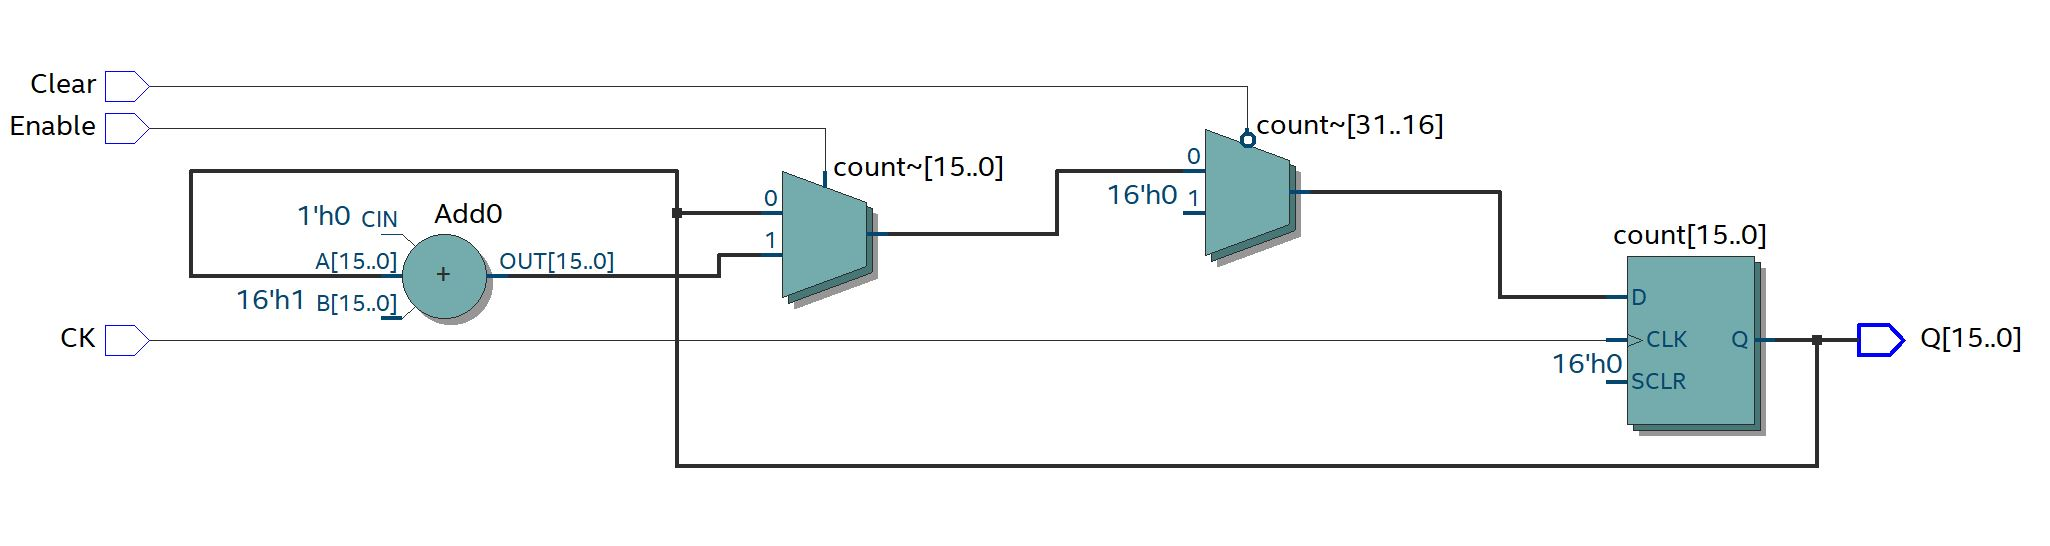
\includegraphics[scale = 0.6]{immagini/RTB3.jpg}
	\caption{RTL view}
\end{figure}

\section{Flashing digits from 0 to 9}
\section{Reaction Timer}
The RT level circuit to implement the reaction timer is shown in $figure x$. Some non standard components are just the implementation of more standard elements in a single component. This was done in order to accelerate the vhdl description of the circuit and simplify the block scheme.
\subsection{millisecond counter}
The purpose of this block is to generate a pulse on the output port connected to $millisecond_signal$ lasting for a clock cycle every millisecond. It has been implemented as a counter that resets and produces a pulse when it reaches the binary equivalent of $50000$. With the DE1 $CLOCK\_50$ clock input at frequency $50MHz$ the circuit counts to $50000$ in $1ms$.
\subsection{counter comparator}
This unit starts to count after it is resetted. Its enable signal is in $and$ with the $millisecond_signal$ to enable the counter only every ms and not every clock cycle. \\When the counter reaches the value set by the inputs $SW_{7-0}$ it stops and the $enable_out$ output is asserted to $1$ until the component is reset.
\subsection{BCD 4digits counter}
This component is made by four $BCDcounters$ connected in a way that they count, modulus 10, numbers up to four digits. Each digit is represented binary using the $BCD$ code and is connected to a decoder driving its respective 7-segments display. \\
As shown in $figure xx$ each $BCDcounter$ has an input $enable$ and output $enable_out$, those signals are connected together between consecutive $BCDcounters$. In particular the $enable_out$ output is asserted to 1 when the digit displayed is $9$ in order to enable the following counter in the next period and properly display the number. The period for the counter is set to $1ms$ by taking the $and$ of each enable input with the $millisecond_signal$.
\subsection{Gated SR latches(non lo sono più,modificare) and connections between blocks}
Two memory elements have been used to implement the requested behavior. 
The $MEM0$ element is responsible to generate the enable signal for the $counter\_comparator$ when occurs pulse of $KEY_0$. The $KEY_0$ input is connected also to the $Asynchronous_clear$ input of the $counter_comparator$ in order to start to count from $0$ when $KEY_0$ is pressed.
\\The $MEM1$ generate a signal useful to stop the $BCD_4digits_counter$ to count and turn off the $LEDR_0$. when $KEY_3$ is pressed. In particular the $LEDR_0$ is active from when the time set by the $SW_{7-0}$ is eplaced (thanks $counter_comparator$) and up to when $KEY_3$ is pressed and the complemented output of $MEM1$ is $0$. The $BCD_4digits_counter$ is active in the same amount of time, but since it has to count every millisecond its enable is in $and$ with the $millisecond_signal$.
\subsection{Testbench}
To be able to verify easily the behaviour of the circuit a new version:"LAB4\_ES5\_tt has been created. This version does not include the 7-segments decoder, therefore the output is directly taken from the $BCD_4digits_counter$. \\
As first thing a clock signal with frequency $f=50MHz$ was generated. 
Then two reaction time measurements cycles are executed with the following parameters:

	\begin{tabular}{lll}
		Cycle & Waiting time & Reaction time \\
		& 3ms          & 17ms          \\
		& 1ms          & 21ms         
	\end{tabular}
\\
\\
Relatively short duration have been chosen in order to make the simulation faster.
\end{document}
